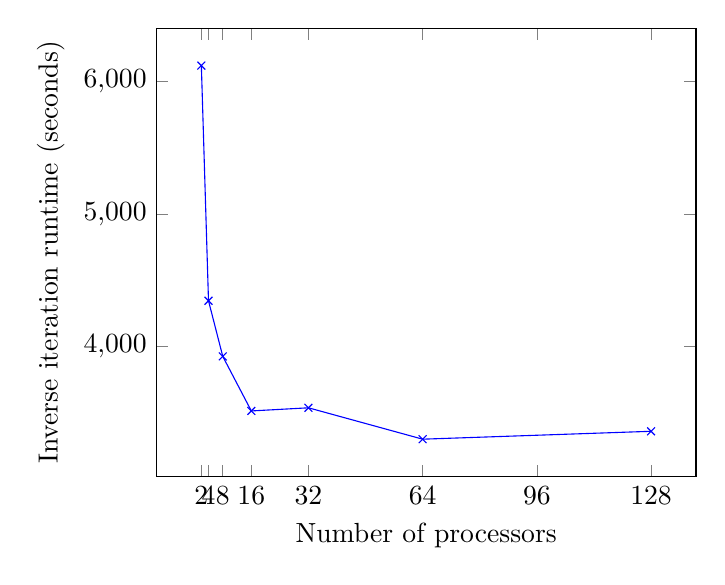
\begin{tikzpicture}
 \begin{axis}[
  xlabel=Number of processors,
  xtick={2, 4, 8, 16, 32, 64, 96, 128},
  ylabel=Inverse iteration runtime (seconds)]
   \addplot[color=blue, mark=x] coordinates {
    (2, 6120.888)
    (4, 4344.505)
    (8, 3924.0755)
    (16, 3512.12)
    (32, 3535.85)
    (64, 3298.803)
    (128, 3358.3466)
   };
 \end{axis}
\end{tikzpicture}

